\documentclass[11pt]{article}
\usepackage[latin1]{inputenc}
\usepackage{amsmath}
\usepackage{amsfonts}
\usepackage{amssymb}
\usepackage{makeidx}
\usepackage{graphicx, array}
\usepackage{pgf,tikz}
\usepackage{tkz-euclide}
\usetkzobj{all}
\pagestyle{empty}
\usepackage{enumerate}
\usepackage[margin = 0.5in]{geometry}
\raggedright

\begin{document}

Name \makebox[3in]{\hrulefill} \hfill Hon. PreCalc P-Set 

\newcommand\bigangle[2][]{% 
    \draw[->,domain=0:#2,variable=\t,samples=200,>=stealth,#1]
      plot ({(\t+#2)*cos(\t)/(4*#2)},
           {(\t+#2)*sin(\t)/(4*#2)}) 
        ;}

\subsubsection*{Angles and Radian Measure  \hfill  \makebox[0.35in]{\hrulefill} / 10}

Convert each to either degrees or radians. Use exact answers only.
\begin{flalign*}
1.  \quad   &   45^\circ        &
2.  \quad   &   \frac{3\pi}{4}  &
3.  \quad   &   555^\circ       &
4.  \quad   &   \frac{\pi}{9}   &
5.  \quad   &   -285^\circ      &&\\[1.25in]
6.  \quad   &   \frac{5\pi}{36} &
7.  \quad   &   -45^\circ       &
8.  \quad   &   \frac{7\pi}{4}  &
9.  \quad   &   140^\circ       &
10. \quad   &   \frac{2\pi}{5}  &&\\[1.25in]
\end{flalign*}

Draw each angle in standard position. Then find a coterminal angle between $0^\circ$ and $360^\circ$ or 0 and $2\pi$ radians for angles outside those ranges.
\begin{flalign*}
11. \quad   &   -220^\circ          &
12. \quad   &   \frac{3\pi}{4}      &
13. \quad   &   70^\circ            &
14. \quad   &   \frac{-11\pi}{3}    &
15. \quad   &   395^\circ           &
16. \quad   &   \frac{-\pi}{2}      &&\\[1.75in]
\end{flalign*}

Find the arc length $s$ and sector area $A$ of each. Exact answers only.
\begin{flalign*}
17. \quad   &   r=5\text{ yd, }\theta = \frac{3\pi}{4}    &
18. \quad   &   r=10\text{ ft, }\theta = \frac{\pi}{2}    &
19. \quad   &   r=2\text{ in, }\theta = 75^\circ    &
20. \quad   &   r=1\text{ m, }\theta = 540^\circ    &&\\[0.15in]
\end{flalign*}


\newpage




The linear velocity $v$ of an object moving around a circle is given by $v=\frac{s}{t}$, while the angular velocity is given as $\omega=\frac{\theta}{t}$. 
\newline\\

21. Find the linear and angular velocities of the problems in 17--20 if the time $t$ is 3 sec. 
\vspace{2.5in}



22. Using the definitions of $v$ and $\omega$ listed above (as well as $s$), show that $v = r\omega$.
\vspace{2in}


23. Two pulleys, one with $r_1$ and the other with radius $r_2$ are connected by a belt. The pulley with radius $r_1$ rotates at $\omega_1$ revolutions per minute. The pulley with radius $r_2$ rotates at $\omega_1$ revolutions per minute.
\newline\\

Show that $\dfrac{r_1}{r_2} = \dfrac{\omega_2}{\omega_1}$.
\newline\\

(\textit{Hint}: The linear speeds of the pulleys are the same because they equal the speed of the belt.)


\newpage


\textbf{Angles and Radian Measure KEY}

\begin{enumerate}
    \item $\frac{\pi}{4}$
    \item $135^\circ$
    \item $\frac{37\pi}{12}$
    \item $20^\circ$
    \item $-\frac{19\pi}{12}$
    \item $25^\circ$
    \item $-\frac{\pi}{4}$
    \item $315^\circ$
    \item $\frac{7\pi}{9}$
    \item $72^\circ$
\end{enumerate}
\vspace{0.25in}
\begin{tabular}{p{0.3\textwidth}p{0.3\textwidth}p{0.3\textwidth}}
11. &   12. &   13. \\

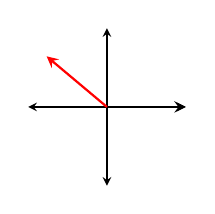
\begin{tikzpicture}
    \draw [<->, >=stealth](-1,0) -- (1,0);
    \draw[<->, >=stealth](0,-1) -- (0,1);
    \draw[->, thick, >=stealth](0,0)--(1,0);
    \draw[->, thick, >=stealth, color=red](0,0) -- (-220:1);
    \bigangle[blue,thick]{-220}    
\end{tikzpicture}   
&
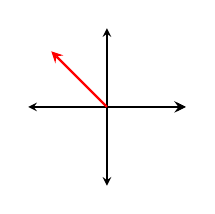
\begin{tikzpicture}
    \draw [<->, >=stealth](-1,0) -- (1,0);
    \draw[<->, >=stealth](0,-1) -- (0,1);
    \draw[->, thick, >=stealth](0,0)--(1,0);
    \draw[->, thick, >=stealth, color=red](0,0) -- (135:1);
    \bigangle[blue,thick]{135}    
\end{tikzpicture}
&
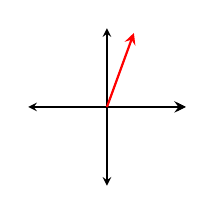
\begin{tikzpicture}
    \draw [<->, >=stealth](-1,0) -- (1,0);
    \draw[<->, >=stealth](0,-1) -- (0,1);
    \draw[->, thick, >=stealth](0,0)--(1,0);
    \draw[->, thick, >=stealth, color=red](0,0) -- (70:1);
    \bigangle[blue,thick]{70}    
\end{tikzpicture}
\\
$140^\circ$ &   &   \\[0.5in]

14. &   15. &   16. \\
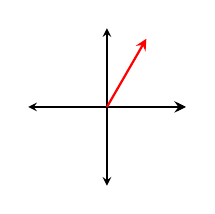
\begin{tikzpicture}
    \draw [<->, >=stealth](-1,0) -- (1,0);
    \draw[<->, >=stealth](0,-1) -- (0,1);
    \draw[->, thick, >=stealth](0,0)--(1,0);
    \draw[->, thick, >=stealth, color=red](0,0) -- (-660:1);
    \bigangle[blue,thick]{-660}    
\end{tikzpicture}
&
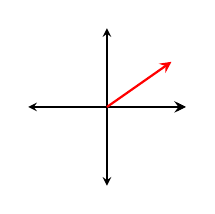
\begin{tikzpicture}
    \draw [<->, >=stealth](-1,0) -- (1,0);
    \draw[<->, >=stealth](0,-1) -- (0,1);
    \draw[->, thick, >=stealth](0,0)--(1,0);
    \draw[->, thick, >=stealth, color=red](0,0) -- (395:1);
    \bigangle[blue,thick]{395}    
\end{tikzpicture}
&
\begin{tikzpicture}
    \draw [<->, >=stealth](-1,0) -- (1,0);
    \draw[<->, >=stealth](0,-1) -- (0,1);
    \draw[->, thick, >=stealth](0,0)--(1,0);
    \draw[->, thick, >=stealth, color=red](0,0) -- (-90:1);
    \bigangle[blue,thick]{-90}    
\end{tikzpicture}
\\
$\left(\frac{\pi}{3}\right)$    &   $35^\circ$  & $\frac{3\pi}{2}$    \\
\end{tabular}
\vspace{0.5in}


17. $s = \frac{15\pi}{4} \text{ yd } \quad A = \frac{75\pi}{8} \text{ sq. yds}$    \\[0.25in]

18. $s = 5\pi \text{ ft } \quad A = 25\pi \text{ sq. ft}$   \\[0.25in]

19. $s = \frac{5\pi}{6} \text{ in } \quad A = \frac{5\pi}{6} \text{ sq. in}$  \\[0.25in]

20. $s = 3\pi\text{ m } \quad A = \frac{3\pi}{2}\text{ sq. m}$






\end{document}
